%!TEX root = ../pres - final.tex

\section{Selección de modelo}

% \begin{frame}{Selección de modelo}
%   \begin{itemize}
%     \itemsep1em    
%     \item Detectar cuántos personas están involucrados en la grabación.

%     \item Hasta ahora se ha considerado que se dispone de esta información, es necesario inferir de alguna manera cuántos interlocutores participan.

%     \item Se propone una técnicas bayesianas como frecuentistas para respaldar la elección realizada.
%   \end{itemize}
% \end{frame}

\begin{frame}{Selección de modelo}{Consideraciones}
  Hay varios aspectos importantes que considerar antes de abordar el problema de selección de modelos (Claeskens y Hjort \cite{Claeskens2010}): 

  \begin{itemize} 
    \itemsep0.8em
    \item \structure{Aproximación:} La realidad observada suele ser mucho más compleja que los modelos propuestos. %No necesariamente existirá un modelo correcto.

    \item \structure{Sesgo-Varianza:} Pocos parámetros a estimar, implican una menor variabilidad; mientras que más con modelos más complejos se reduce el sesgo.

    \item \structure{Parsimonia:} 'El principio de parsimonia' o navaja de Ockham.

    \item \structure{Contexto:} En algunos contextos puede ser más interesante encontrar los parámetros subyacentes del modelo e interpretarlos, mientras que en otros puede bastar con obtener respuesta a las problema planteado.
  \end{itemize}
\end{frame}

\begin{frame}{Funciones de penalización}
  \begin{itemize} 
    \itemsep1em
    \item
    Una estrategia sencilla para la selección de modelo es elegir el candidato con la más grande probabilidad dados los datos. 

    \item
    No siempre es un criterio lo suficientemente bueno para la comparación de modelos (sobre-ajuste del modelo). 

    \item 
    Utilizar una función que además de la verosimilitud del modelo, considere su complejidad
  \end{itemize}
\end{frame}    

\subsection{BIC}

\begin{frame}{Criterio de Información Bayesiano}
  \begin{itemize} 
    \itemsep1em
    \item 
    Cuando hay varios modelos candidatos, una estategia bayesiana se encargaría de seleccionar el modelo que a posteriori sea más probable. 

    \item
    Calcular la probabilidad posterior de cada uno de los modelos y luego seleccionando aquél modelo cuya probabilidad sea la mayor.
%  \end{itemize}
%\end{frame}        

%\begin{frame}{Criterio de Información Bayesiano}
%  \begin{itemize} 
    %\itemsep1em
    \item
    Sean $\mathcal{M}_1, ..., \mathcal{M}_k$ los modelos propuestos, y sea $\mb{X} = \lbrace x_1, ..., x_n \rbrace $ el vector de datos observados. La probabilidad a posteriori para cada modelo se puede calcular como sigue: 
    \begin{equation}
    P(\mc{M}_j \,|\, \mb{X}) \equiv \frac{P(\mc{M}_j)}{f(\mb{X})} 
      \int_{\Theta_j} f(\mb{X} \,|\, \mc{M}_j, \theta_j) \pi(\theta_j \,|\, \mc{M}_j) d\theta_j
    \label{eqn:4-1}
    \end{equation}
    % donde $\Theta_j$ es el espacio de parámetros al que pertenece $\theta_j$. Además, $f(\mb{X} \,|\, \mc{M}_j, \theta_j)$ es la verosimilitud $\mc{L}_{j}(\theta_j)$ de los datos, dado al modelo $j$ y sus parámetros; mientras que $ \pi(\theta_j \,|\, \mc{M}_j) d\theta_j$ representa la densidad a priori de $\theta_j$ dado el modelo $\mc{M}_j$; $P(\mc{M}_j)$ es la probabilidad a priori para el modelo $j$-ésimo y $f(\mb{X})$ es la verosimilitud de los datos.
  \end{itemize}
\end{frame}    

\begin{frame}{Criterio de Información Bayesiano}
  \begin{itemize} 
    \itemsep1em
    \item 
    La verosimilitud incondicional de los datos se puede calcular como sigue: 
    \begin{equation}
    f(\mb{X}) = \sum_{j=1}^k P(\mc{M}_j) \lambda_{n, j}(y)
    \label{eqn:4-2}
    \end{equation}
    donde 
    \begin{equation}
    \lambda_{n, j} = \int_{\Theta_j} \mc{L}_{n, j}(\theta_j) \pi(\theta_j \,|\, \mc{M}_j) d\theta_j.
    \label{eqn:4-3}
    \end{equation}

    \item
    La ecuación \eqref{eqn:4-3} representa la verosimilitud marginal de los datos para el modelo $\mc{M}_j$ integrada con respecto a $\theta_j$ sobre es espacio de parámetros $\Theta_j$ correspondiente.
  \end{itemize}
\end{frame}        


\begin{frame}{Criterio de Información Bayesiano}
  \begin{itemize} 
    \itemsep1em
    \item 
    Ahora, si se define 
    \begin{equation}
    BIC_{n, j}^{exact} \equiv 2 log(\lambda_{n, j}(\mb{X}))
    \label{eqn:4-4}
    \end{equation}
    por lo que \eqref{eqn:4-1} se podría reescribir como sigue: 
    \begin{equation}
    P(\mc{M}_j \,|\, \mb{X}) = \frac{ P(\mc{M}_j)  exp(\frac{1}{2} BIC_{n, j}^{exact}) }
    { \sum_{i=1}^k  P(\mc{M}_i) exp(\frac{1}{2} BIC_{n, i}^{exact}) }
    \label{eqn:4-5}
    \end{equation}

    \item 
    El cálculo de los diferentes $BIC_{n, j}^{exact}$ es difícil de estimar numéricamente, además de que se necesitan las probabilidades a priori para todos los modelos y todos los parámetros; por lo que se usará una expresión similar que sea práctica y mucho más eficiente.
  \end{itemize}
\end{frame}        


\subsection{Bootsrap}

\begin{frame}{Bootstrap}
  \begin{itemize} 
    \itemsep1em
    \item 
    \structure{Bootstrap} es una técnica estadística que nos permite tener noción sobre qué tan precisa es alguna medida muestral estimada. 

    \item Permite aproximar la distribución de muestreo de casi cualquier estadístico, usando métodos sencillos pero computacionalmente intensivos. 

    \item Como menciona Persi~et.al~\cite{Diaconis1983}, esta técnica fue desarrollada en 1978 por Efron~\cite{Efron1978}, quien generalizó el método de \textit{Jacknife}.

  \end{itemize}
\end{frame}        

\begin{frame}{Bootstrap no paramétrico}
  \begin{itemize} 
    \itemsep1em
      \item
      Se tiene que ajustar un modelo a un conjunto de datos. Sea este conjunto de entrenamiento $\mb{Z} = (z_1, z_2, ..., z_N)$ donde $z_i = (x_i, y_i)$ y son independientes con distribución $F$. 

      \item
      Como $\mb{Z}$ es una muestra finita no se conoce tal cual la distribución $F$, 

      \item
      Se estimarpa una función empírica $\hat F$ donde a cada observación $z_i$ se le asigna un peso $\frac{1}{N}$ en la densidad.
    \end{itemize}
\end{frame}        

\begin{frame}{Bootstrap no paramétrico}
  \begin{itemize} 
    \itemsep1em
      \item
      Seleccionar de forma aleatoria y con reemplazo de $\hat{F}$ un conjunto de datos del mismo tamaño que el conjunto original. 

      \item A este conjunto se le denotará $\mb{Z}^{*}_1$. Este proceso de selección se realiza $B$ veces, produciendo $B$ conjuntos bootstrap $\mb{Z}^{*}_{\cdot} = \lbrace \mb{Z}^{*}_1, \mb{Z}^{*}_2, ..., \mb{Z}^{*}_B \rbrace$. 

      \item Para cada uno de estos conjuntos resultantes, se volvera a ajustar el modelo, y se examinará el comportamiento de los ajustes para las respuestas obtenidas, obteniendo lo que se conoce como réplica bootstrap.
    \end{itemize}
\end{frame}        

\begin{frame}{Bootstrap no paramétrico}
  \begin{figure}[tp]
    \centerline
    {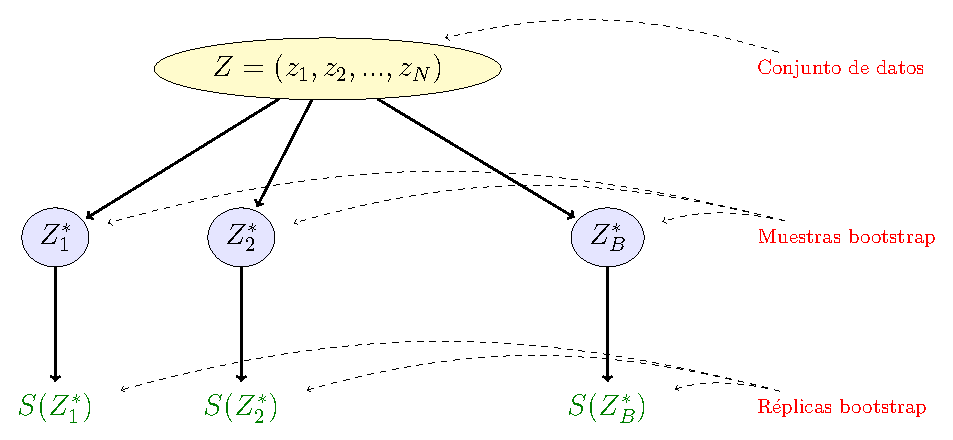
\includegraphics[width=0.9\linewidth]{gfx/bootstrap}}
    \label{fig:bootesq}
  \end{figure}
\end{frame}        

\begin{frame}{Bootsrap paramétrico}
  \begin{itemize} 
    \itemsep1em
    \item El bootstrap clásico es no paramétrico, y se vale únicamente del conjunto observado para a partir de ahí estimar la función de distribución empírica. 

    \item En el caso que nos interesa, se cuenta con un modelo paramétrico que ha sido ajustado a los datos, usualmente por MLE. 

    \item A partir de este modelo ajustado es que se muestrea. Al igual que en con la técnica no paramétrica, se suelen generan muestras de datos del mismo tamaño que el conjunto original. 

    \item Luego, para cada nueva conjunto bootstrap $\mb{Z}^{*}_b$ muestreado se calcula el estadístico de nuestro interés. Éste proceso de muestreo se repite igualmente una gran cantidad de veces. 
  \end{itemize}
\end{frame}

\begin{frame}{Selección de modelo usando BIC}
  \begin{itemize} 
    \itemsep1em

    \item Puesto que consideramos que dentro de nuestro espacio de modelos propuestos se encuentra el modelo solución, resulta más natural usar BIC (cita).

    \item Esta función de penalización se calcula de la siguiente manera: 
    \begin{equation}
    BIC(\mc{M}) = 2 \mc{L}_{max}(\mc{M}) - (log N ) dim(M)
    \end{equation}
    para cada modelo $\mc{M}$, donde $dim(M)$ es el número estimado de parámetros libres que le corresponden, y $N$ es el tamaño de nuestra muestra de datos. 

    \item Por otra parte, $\mc{L}_{max}(\mc{M})$ es la máxima log-verosimilitud obtenida para el modelo $\mc{M}$ después de realizar un número $HMM_{MAX}$ de simulaciones, para evitar que en algún caso el algoritmo de estimación se quede atorado en un máximo local.
  \end{itemize}
\end{frame}


\begin{frame}{Selección de modelo usando BIC}
  \begin{itemize} 
    \itemsep1em

    \item Para estimar el número de parámetros libres de nuestro modelo, se consideran todas las probabilidades que rigen al HMM:
    \begin{itemize} 
      \itemsep0.8em
      \item Matriz a priori o inicial
      \item Matriz de transición entre los interlocutores
      \item Matriz de emisión de cada persona para todo el diccionario de palabras
    \end{itemize}

    \item Este tipo de función de penalización nos permite seleccionar de entre un conjunto de modelos propuestos (que pueden ser muchos) al modelo o los modelos con mayor probabilidad de ser los correctos. 

  \end{itemize}
\end{frame}

\begin{frame}{Selección de modelo usando bootstrap con likelihood ratio testing}
  \begin{itemize} 
    \itemsep1em

    \item Se utilizará la técnica bootstrap paramétrico, pues mediante el algoritmo EM es fácil obtener el modelo parametrizado. 

    \item Usualmente se compararán dos modelos adyacentes, es decir, el modelo $\mc{M}_d$ de $d$ estados contra el modelo $\mc{M}_{d+1}$ de $d+1$ estados ocultos.

    \item Se usa el estadístico LLR que corresponde a la diferencia de las log-verosimilitudes de dos modelos
      \begin{equation}
        LLR^{(d)}_{obs} = \log \frac{L(\hat \theta^{(d+1)}; y_{1:n})}{L(\hat \theta^{(d)}; y_{1:n})} =
          \log L(\hat \theta^{(d+1)}; y_{1:n}) - 
          \log L(\hat \theta^{(d)}; y_{1:n})
      \end{equation}
  \end{itemize}
\end{frame}

\begin{frame}{Selección de modelo usando bootstrap con likelihood ratio testing}
  \begin{itemize} 
    \itemsep1em
    \item Para calcular el MLE de un modelo, se estimó la verosimilitud varias veces con diferentes parámetros iniciales aleatorios. 

    \item Se iteró el algoritmo EM hasta convergencia, un numero $iter_{hmm}$ fijo de iteraciones, esto para evitar el estancamiento del algoritmo en un máximo local, y obtener así una buena estimación de la máxima verosimilitud del modelo.

    \item Se usó entonces como MLE del modelo la máxima verosimilitud correspondiente a los mejores parámetros estimados y que se denotó por $LLR_{obs}$.
  \end{itemize}
\end{frame}
